\author{Tadd\"aus Nauheimer}
\chapter{Aufgaben Typen}

Hier werden die verschiedenen Aufgabentypen beschrieben.
Es ist wichtig, dass beim Ausw\"ahlen der Aufgaben der richtige Typ gesetzt wird.

\section{Number}

Dieser Aufgabentyp sollte gew\"aehlt werden, wenn die Aufgabe nur eine Zahl ergeben soll. 
Dabei kann eine einzelne oder mehrstellige Zahl angegeben werden, allerdings keine Dezimalzahlen oder negative Werte.

\subsection{Beispiele}

Funktionierende Werte:

\begin{itemize}
	\item 0
	\item 5
	\item 100
	\item 123451125158915815
\end{itemize}

\textbf{Nicht} funktionierende Werte:

\begin{itemize}
	\item -2
	\item - 2
	\item 3.5
	\item 3,5
\end{itemize}

\section{Checkboxes}

Dieser Aufgabentyp soll gesetzt sein, wenn es sich bei der Aufgabe um eine Single Choice Aufgabe handelt.
Hier sollen \textbf{nur} die Boxen an sich markiert werden.

\subsection{Beispiele}

Richtig:
\begin{figure}[H]
	\centering
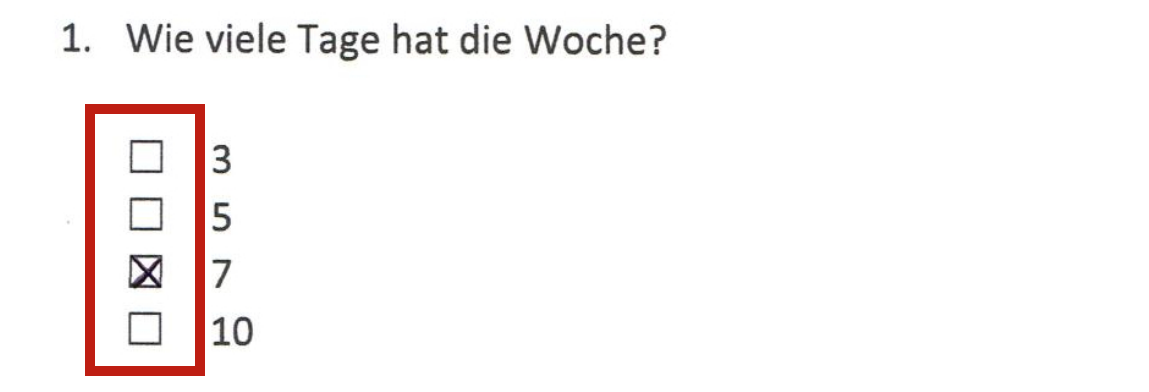
\includegraphics[width=\textwidth]{correct_selected.png}
\end{figure}
\par\rule{\textwidth}{0.5pt}

Falsch:

\begin{figure}[H]
	\centering
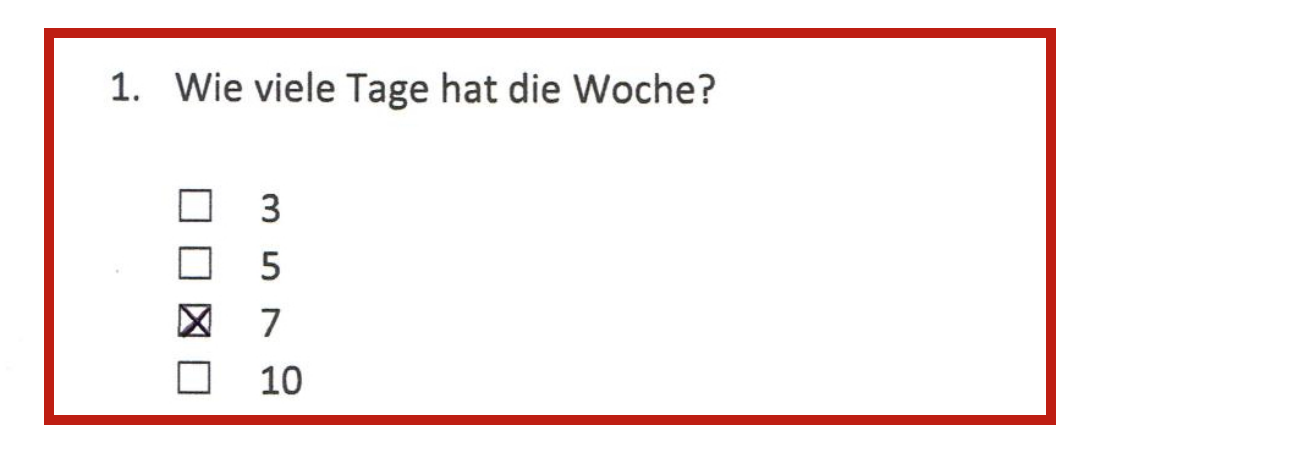
\includegraphics[width=\textwidth]{too_much_selected-task.png}
\end{figure}

\begin{figure}[H]
	\centering
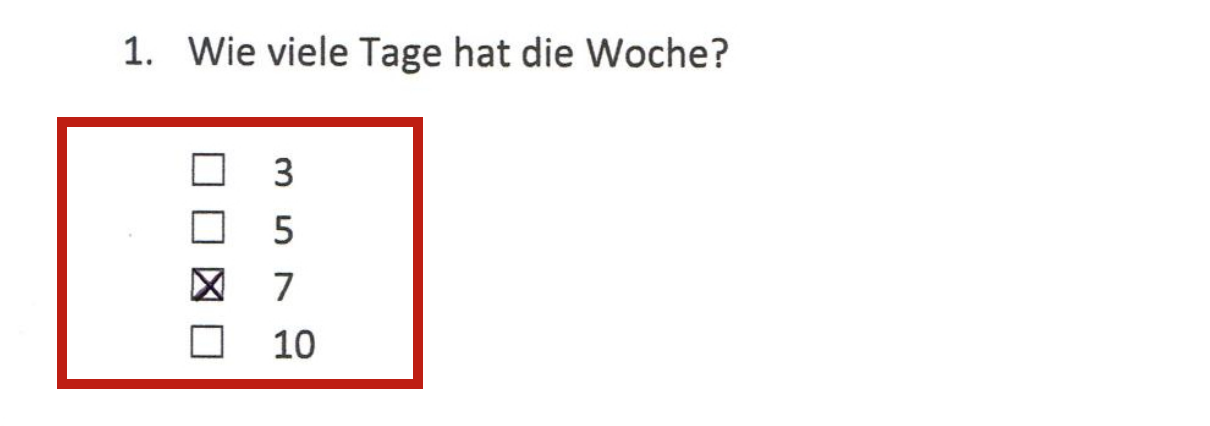
\includegraphics[width=\textwidth]{too_much_selected-options.png}
\end{figure}



\section{Text}

Dieser Aufgabentyp soll verwendet werden, wenn es sich um Worte/Text handelt.
Dabei k\"onnen in dem Text auch Zahlen vorkommen.
Zeichen die erkannt werden sind:

\begin{itemize}
	\item a bis z (Gro{\ss}buchstaben werden erkannt aber in Kleinbuchstaben umgewandelt)
	\item 0 bis n
	\item Leerzeichen
\end{itemize}

H\"aufig vorkommende Zeichen die \textbf{nicht} erkannt werden:

\begin{itemize}
	\item .
	\item ,
	\item \"a \"o \"u
\end{itemize}

\section{Text-no-number}

Dieser Aufgabentyp ist daf\"ur gemacht, Text besser zu erkennen.
Als Kompromiss kann dieser Aufgabentyp jedoch keine Zahlen erkennen.
Die Zeichen die in diesem Typ erkannt werden k\"onnen sind identisch mit dem Typ "Text" exklusive der Zahlenerkennung.
